The performance evaluation involves investigating a shared-memory performance
scaling on the 64 core machine, togian, and a comparison in shared-memory
performance between GMCF and MPI.

\subsection{Evaluation Methodolody}

To ensure direct comparisons between GMCF and MPI performance scaling can be
made, the evaluation methodology used is identical to the one discussed in
Section~\ref{sec:mpievaluationmethodology} bar two differences. The first is
that GMCF uses threads for parallelisation whereas MPI uses processes. The
second is that GMCF performance scaling does not include 63 and 64 instances of
the LES. This is due to a temporary implementation detail discussed in
Section~\ref{sec:GMCFInvestigation}. Given the performance characteristics of
both MPI and GMCF these two omissions are insignificant in showing the
performance scaling of GMCF in comparison to MPI.

\subsection{Shared-memory parallelisation}

The shared-memory parallelisation evaluation was conducted on the same machine
as for the MPI shared-memory parallelisation evaluation, togian.

\begin{figure}
    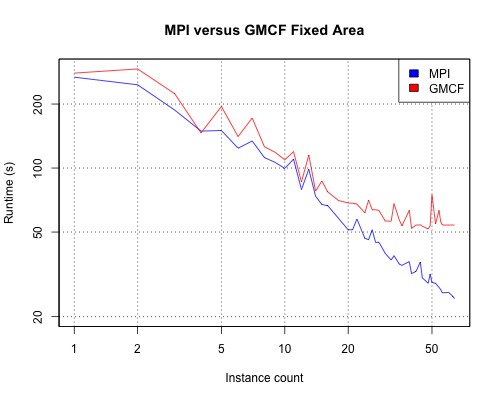
\includegraphics[width=0.5\textwidth]{graphs/GMCF-MPI-fixed-area.png}
    \caption{MPI versus GMCF Fixed Area}
    \label{fig:gmcfmpifixedarea}
\end{figure}

\begin{figure}
    \includegraphics[width=0.5\textwidth]{graphs/GMCF-MPI-expanding-area.png}
    \caption{MPI versus GMCF Expanding Area}
    \label{fig:gmcfmpiexpandingarea}
\end{figure}

Figure~\ref{fig:gmcfmpifixedarea} shows the performance scaling for a fixed
area. MPI's best runtime over all process counts is 24.3 seconds with GMCF's
best runtime over all thread counts is 51 seconds. This means GMCF is 2.1x
slower than MPI which is a significant difference and thus indicates GMCF
requires further work to improve performance for communication involving small
transfers.

Figure~\ref{fig:gmcfmpiexpandingarea} shows the performance scaling for an
expanding area. The results in this case are much more promising with little
difference between runtimes for less than 32 instances of the LES. At greater
numbers of processes, MPI settles to around 220 seconds with GMCF settling at
around 234 seconds. This means the performance differential is around 6\% making
GMCF highly competitive with MPI for larger transfers. With the expanding area
evaluation involving a more likely scenario where computational power is used to
simulate at higher resolutions or over larger areas, this result is more
indicative of realistic performance characteristics.

Overall, MPI may be faster than GMCF but the GMCF performance results are highly
competitive. The MPICH library is the initial implementation of the MPI 1.x
standard so is around two decades old. Throughout its existence, it has also
acted as a high quality reference implementation of the latest MPI standard.
This makes MPICH a well thought out and mature library. GMCF's implementation
began in August 2014, less than a year ago and the primary work was aimed at
model coupling, not parallelism of a single model. As such, as GMCF matures it
can be expected that the performance gap will narrow with the potential for GMCF
to overtake MPI in shared-memory benchmarks since MPIs focus has been on
distributed-memory parallelism, potentially making some implementation details
suboptimal for shared-memory parallelism.
